\subsection{Солнечное время. Уравнение времени}
\term{Истинные солнечные сутки}~--- промежуток времени между двумя последовательными одноимёнными кульминациями Солнца.

\term{Истинное солнечное время}~--- промежуток времени между нижней кульминацией Солнца и любым другим его положением. Рассчитывается по следующей формуле:
\begin{equation}
T_{\text{ист}}=t_{\text{сол}}+12^h,
\end{equation}
где $t_{\text{сол}}$~--- часовой угол Солнца.

\term{Среднее солнечное время} ($T_m$)~--- промежуток времени между нижней кульминацией среднего Солнца и любым другим его положением. \imp{Среднее Солнце}~--- точка небесной сферы, которая равномерно движется по небесному экватору, совершая полный оборот вокруг точки весеннего равноденствия за тропический год. Зная долготу наблюдателя, нетрудно вычислить среднее солнечное время:
\begin{equation}
T_m = \text{UTC} + \lambda,
\end{equation}
где UTC~--- всемирное время равное среднему солнечному времени в Гринвиче.

\term{Поясное время}~--- местное среднее солнечное время на срединном меридиане географического часового пояса. В России также установлено декретное время, которое на 1 час больше поясного.


\term{Уравнение времени}~--- разница между истинным солнечным временем и средним солнечным временем:
\begin{equation}
\eta=T_{\text{ист}}-T_m
\end{equation}


\begin{figure}[!h]
\centering
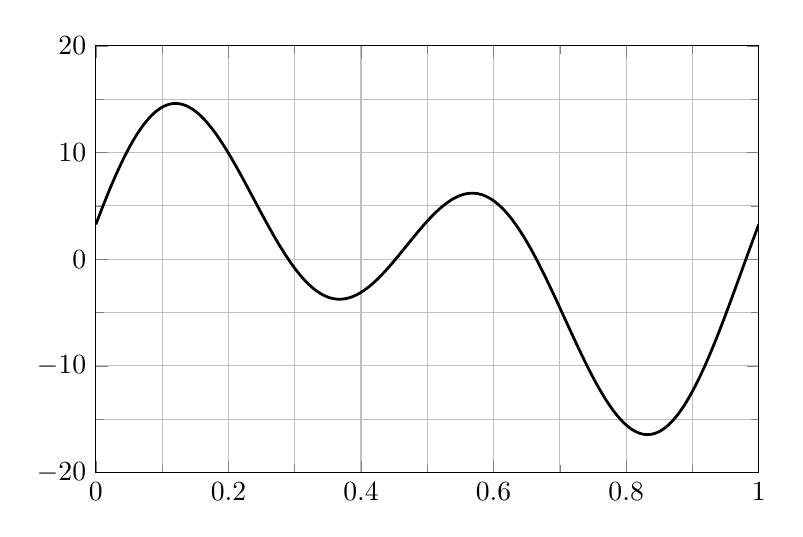
\begin{tikzpicture}
 		 \begin{axis}[width=10cm, 
 		 height=7cm, no markers, grid = both, xmax = 1, xmin = 0, ymax = 20, ymin = -20,
 		  minor x tick num = 1,
 minor y tick num = 1]
%  			  \addplot [black, smooth, line width=1pt] table[x=x,y=y]{data/time_eq.txt};
  			  \addplot [domain=0:1, samples = 100, black, smooth, line width=1pt] {7.53 * cos(360*(x - 81/365)) + 1.5 * sin(360*(x - 81/365)) - 9.87 * sin(2*360*(x - 81/365))};
		 \end{axis}
	\end{tikzpicture}
\caption{График уравнения времени}
\end{figure}